\section{Introduction}~\label{sec:introduction}
In this paper, we consider the problem of real-time reliable trajectory execution for humanoid robots. A precise localization on a humanoid robot is both crucial to achieve reliable trajectory execution and challenging due to humanoid robots specific features. We propose a novel control architecture for humanoid robots where the current localization is used by the robot controller and planner trajectory. The objective of this work is to localize the humanoid robot HRP-2~\cite{Kaneko04icra} while it is navigating through an indoor environment.

Localization is crucial on a humanoid robot as its position cannot be controlled directly. Legs motion are planned under the assumption that all contacts will be perfect (i.e.\ no friction) during the movement. This is not the case in practice and leads to execution errors which cannot be ignored. Moreover, reactive control
algorithms rely on simplified dynamics models such as the \textit{Linear Inverted Pendulum} model~\cite{Kajita01iros}. These imply a gap between the generated motion and the executed one. Therefore, localization is necessary to ensure a consistent robot behavior.

However, localization on a humanoid robot is challenging. Mobile robots odometry can be computed using wheel encoders and give a reasonable hint on the current robot motion. 2D maps can also be used to simplify the navigation through indoor environments. This is not the case on a legged robot on which 3D localization is required and where no encoder based reliable odometry exists.
%
\begin{figure}[ht]
  \begin{center}
    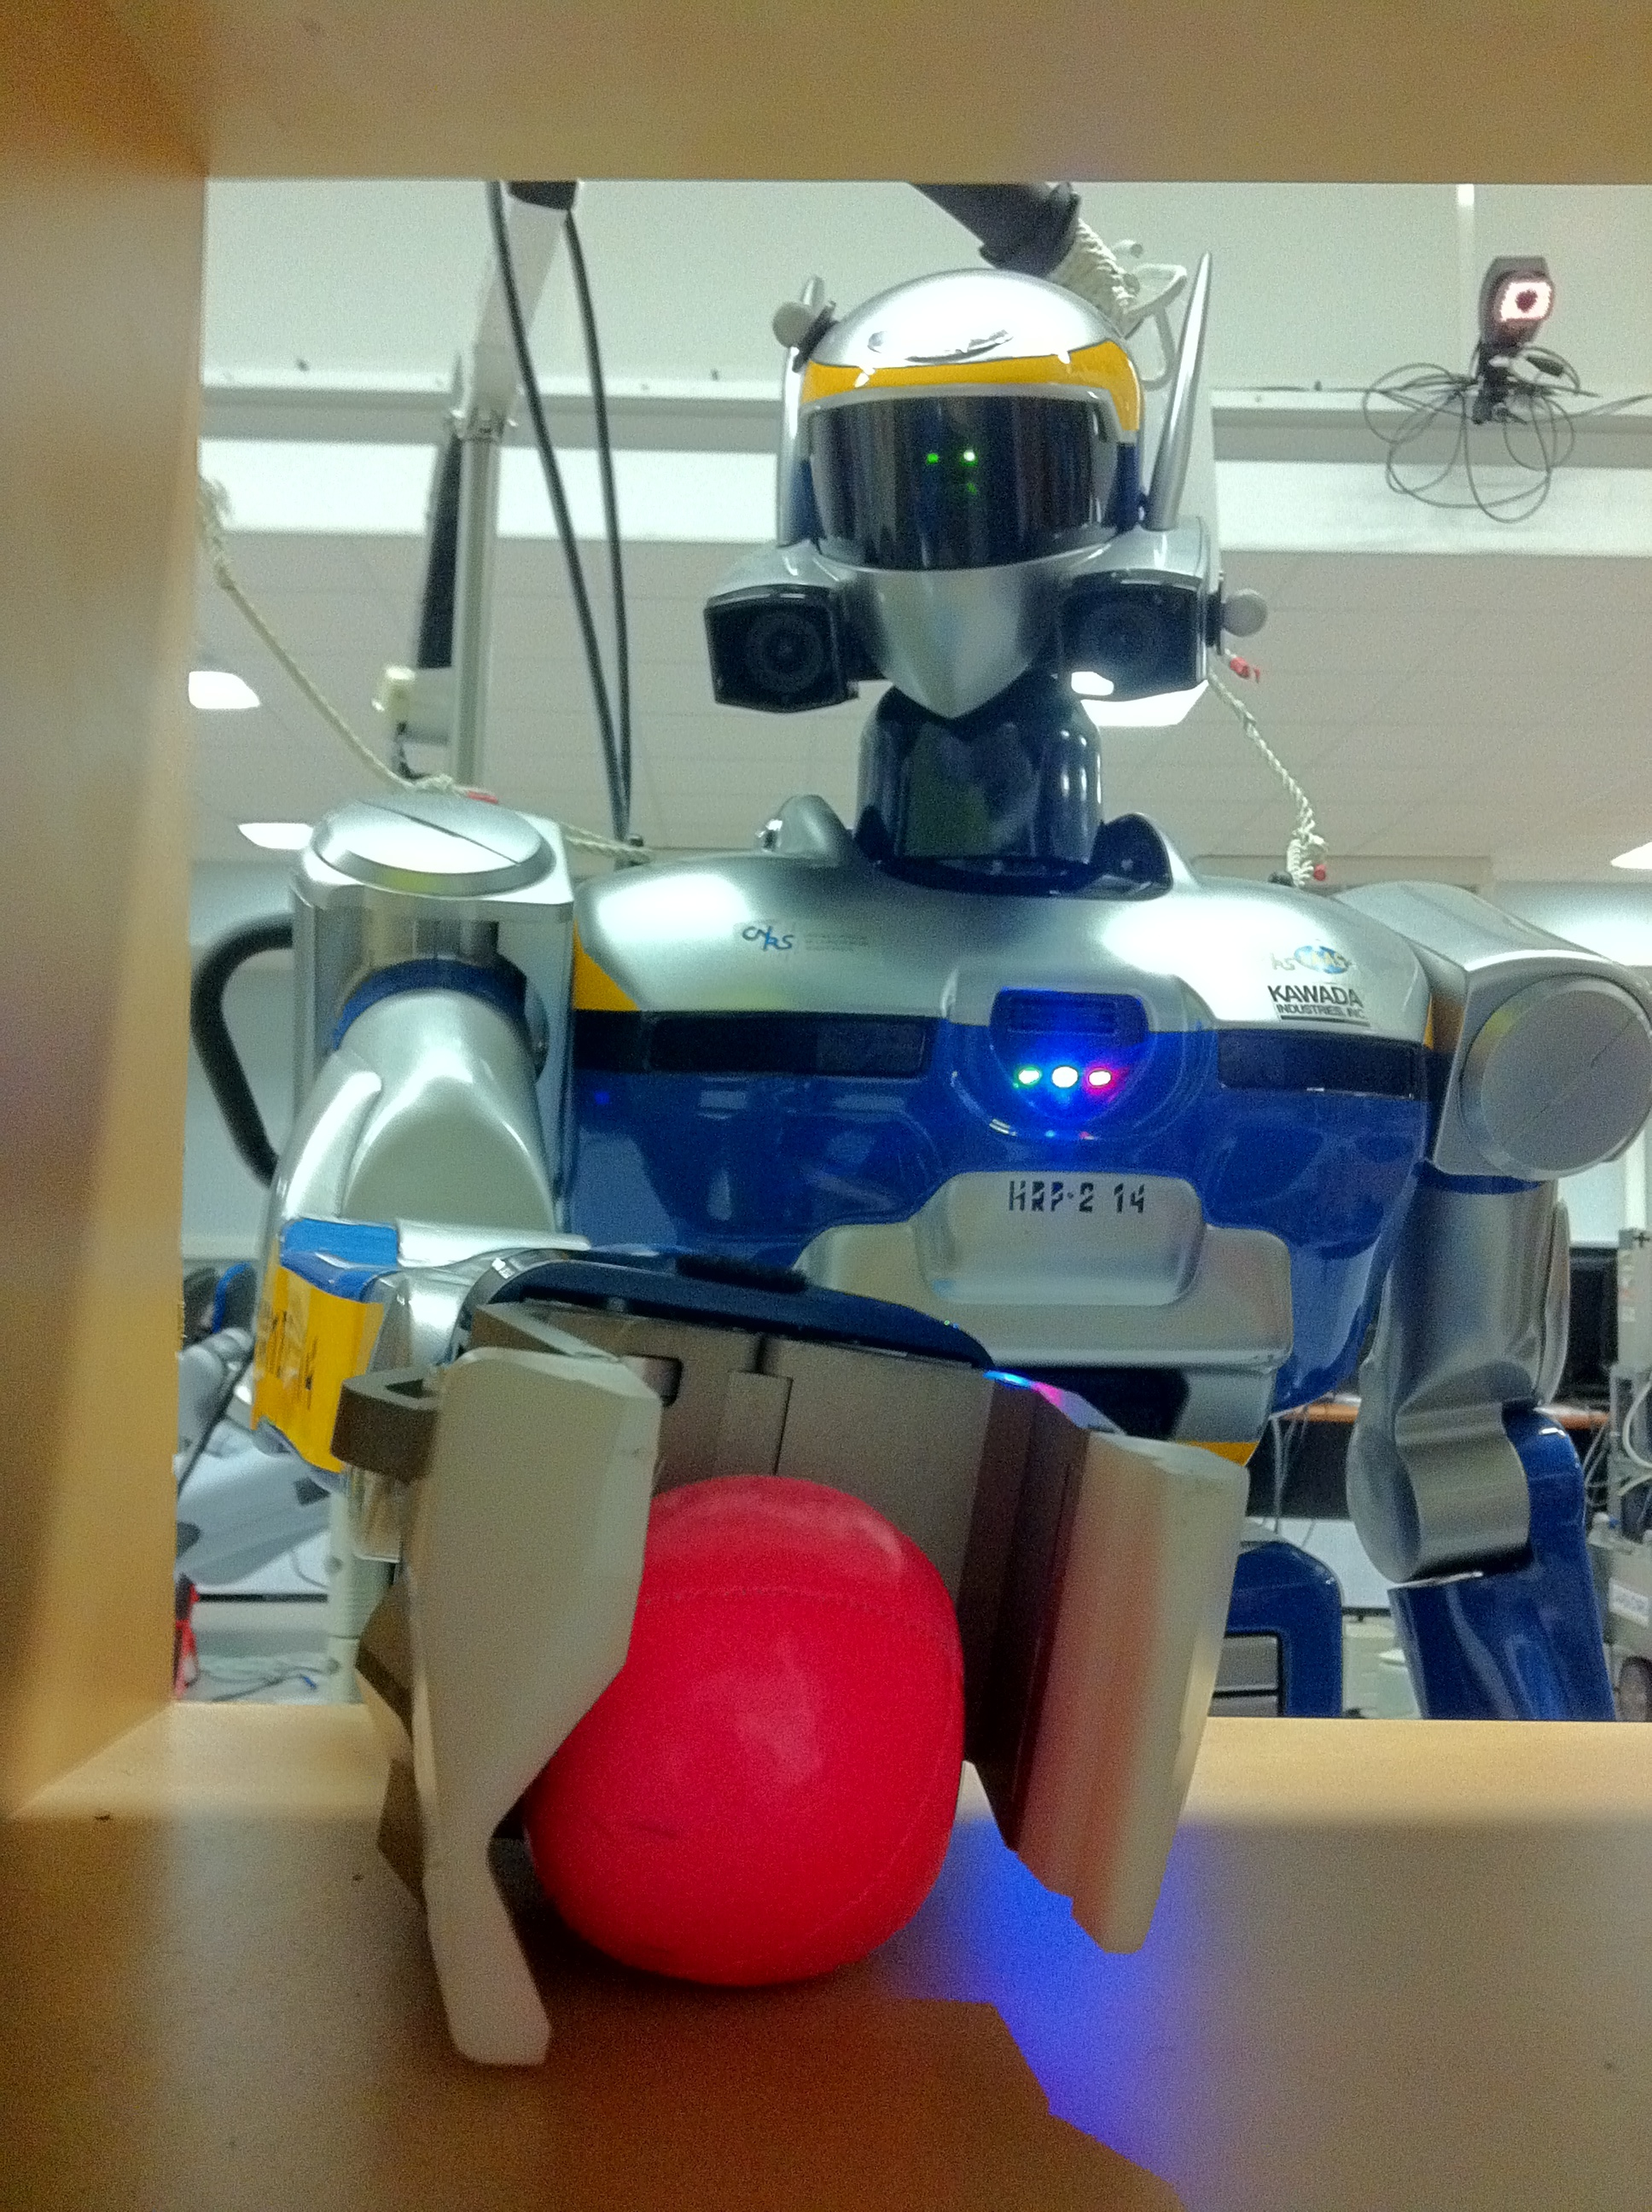
\includegraphics[width=.9\linewidth]{images/demo1.JPG}
  \end{center}
  \caption{HRP-2 dropping a ball on a shelf after having navigated through an indoor environment. Navigation followed by manipulation are typical scenarios where walking drift can prevent a task from being accomplished.\label{fig:xp_final}}
\end{figure}
%
All these reasons make localization a cornerstone of reliable trajectory execution on humanoid robots. To obtain an accurate localization of the robot in the environment, we employ fast vision-based localization techniques~\cite{Alcantarilla10icra} that assume that a prior 3D map of the environment exists. By means of \textit{visibility prediction}~\cite{Alcantarilla11icra}, a fast and robust data association between a large map of 3D points and perceived 2D features in the image can be performed very efficiently. Firstly, the 3D map of the environment is computed by using visual Simultaneous Localization and Mapping~(SLAM)~\cite{Davison07pami,Konolige08tro} techniques.

In this article, the past results in vision processing on humanoids robots are presented in Section~\ref{sec:related}. Section~\ref{sec:architecture} details how the vision is linked to the robot
controller via our proposed control scheme. The vision-based localization algorithm is described in detail in Section~\ref{sec:vision}. The experimental results are discussed and compared to motion capture data
in Section~\ref{sec:results}. Finally, conclusions and future work are described in Section~\ref{sec:conclusions}.
\PFA{Minor: I normally like writing Section instead of anything.}
%%% Local Variables:
%%% ispell-local-dictionary: "american"
%%% LocalWords:  odometry HRP roadmap
%%% End:
